\chapter{Esecuzione}
\label{ch:results}
Qui vengono confrontati i due algoritmi REPTree e RIPPER/JRip. Entrambi hanno sfruttato una \textit{10-fold cross validation}.

\section{Risultati su \texttt{German Credit}}

\begin{mdframed}[frametitle=Esecuzione REPTree]
	\footnotesize\verbatiminput{results/reptree/german_credit.reptree}
\end{mdframed}

\begin{sidewaysfigure}
	\thisfloatpagestyle{empty}
	%	
\includegraphics[width=\textwidth, height=\textheight]{results/reptree/gc.pdf}
	\makebox[\textwidth]{
\includegraphics[width=1.4\textwidth, height=.4\textheight]{results/reptree/gc.pdf}}
	\caption{Modello di REPTree}
\end{sidewaysfigure}

\pagebreak

\begin{mdframed}[frametitle=Esecuzione JRip]
	\footnotesize\verbatiminput{results/jrip/german_credit.jrip}
\end{mdframed}

\vspace{-2em}
\begin{mdframed}[frametitle=Regole]
	\begin{adjustwidth}{.25\linewidth}{}
		\verbatimtabinput{results/jrip/german_credit.rules}
	\end{adjustwidth}
\end{mdframed}
%\begin{adjustwidth}{-3em}{}
%	\footnotesize\verbatimtabinput{results/jrip/german_credit.rules}
%\end{adjustwidth}



\pagebreak

\section{Risultati su \texttt{Image Segmentation}}

\begin{mdframed}[frametitle=Esecuzione REPTree]
	\scriptsize\verbatiminput{results/reptree/segment.reptree}
\end{mdframed}

\begin{figure}[htb]
	\makebox[\textwidth]{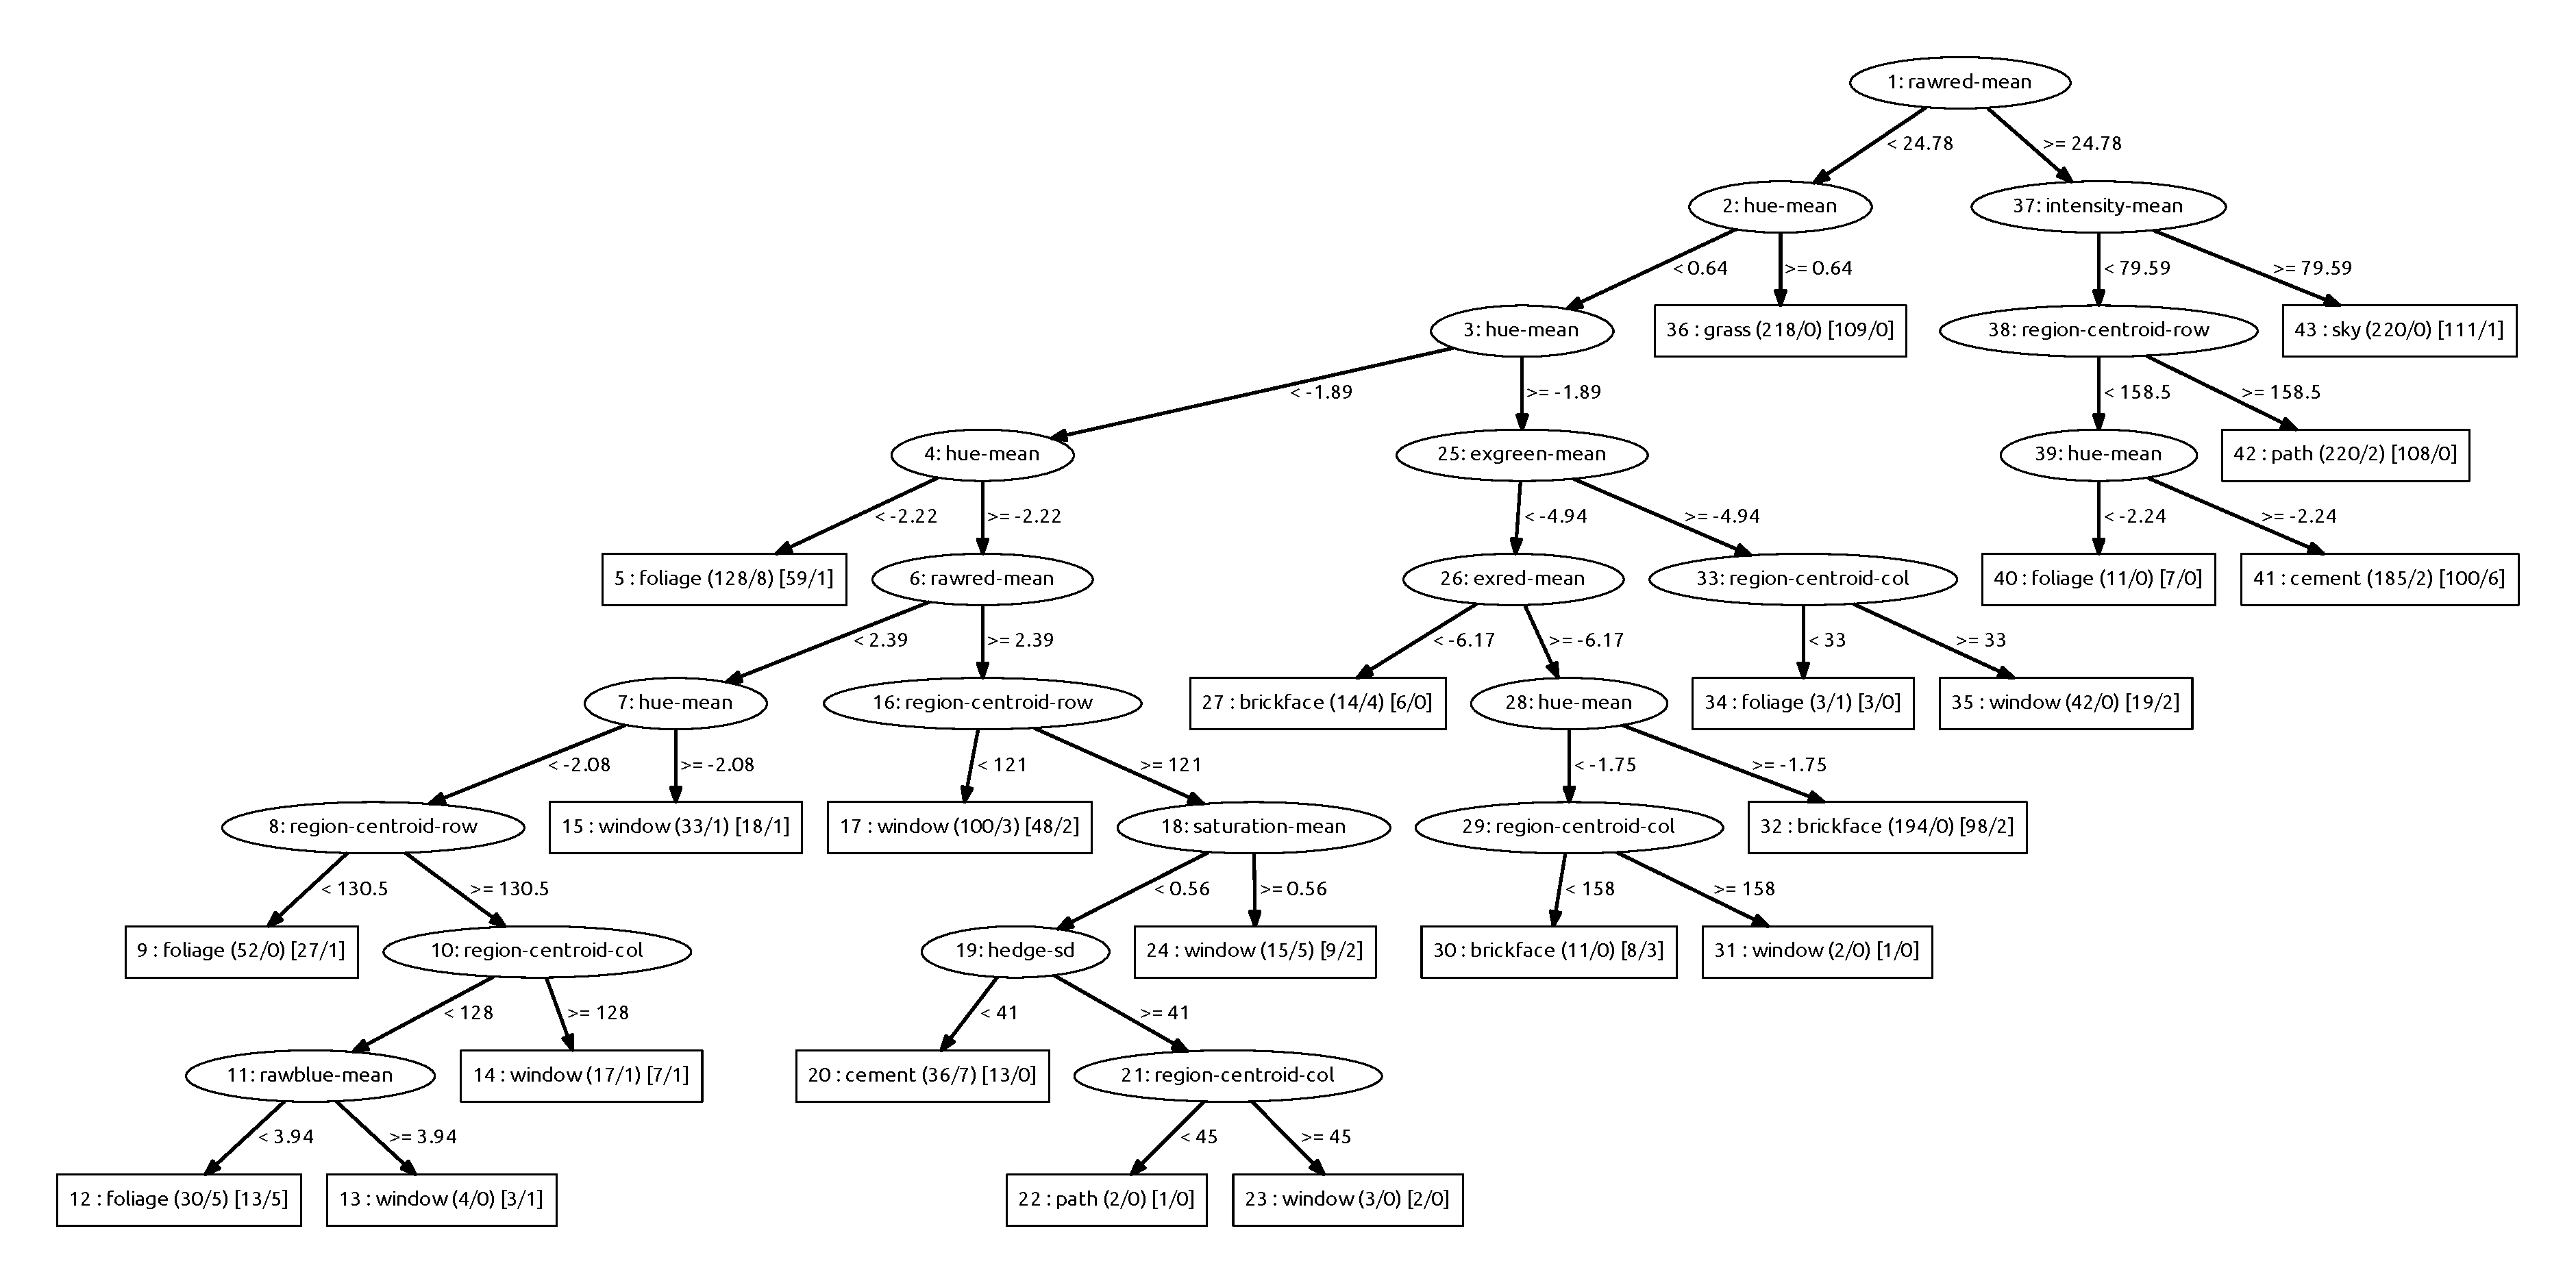
\includegraphics[width=1.55\textwidth]{results/reptree/segment.pdf}}
	\caption{Modello di REPTree}
\end{figure}

\begin{mdframed}[frametitle=Esecuzione JRip]
	\scriptsize\verbatiminput{results/jrip/segment.jrip}
\end{mdframed}

%\begin{adjustwidth}{-8em}{}
%	\scriptsize\verbatimtabinput{results/jrip/segment.rules}
%\end{adjustwidth}

\vspace{-2em}
\begin{mdframed}[frametitle=Regole]
	\begin{adjustwidth}{.33\linewidth}{}
		\scriptsize\verbatimtabinput{results/jrip/segment.rules}
	\end{adjustwidth}
\end{mdframed}



\pagebreak

\section{Risultati su \texttt{Vehicle Silhouettes}}

\vspace{-1em}
\begin{mdframed}[frametitle=Esecuzione REPTree]
	\scriptsize\verbatiminput{results/reptree/vehicle.reptree}
\end{mdframed}

\begin{figure}[htb]
	\makebox[\textwidth]{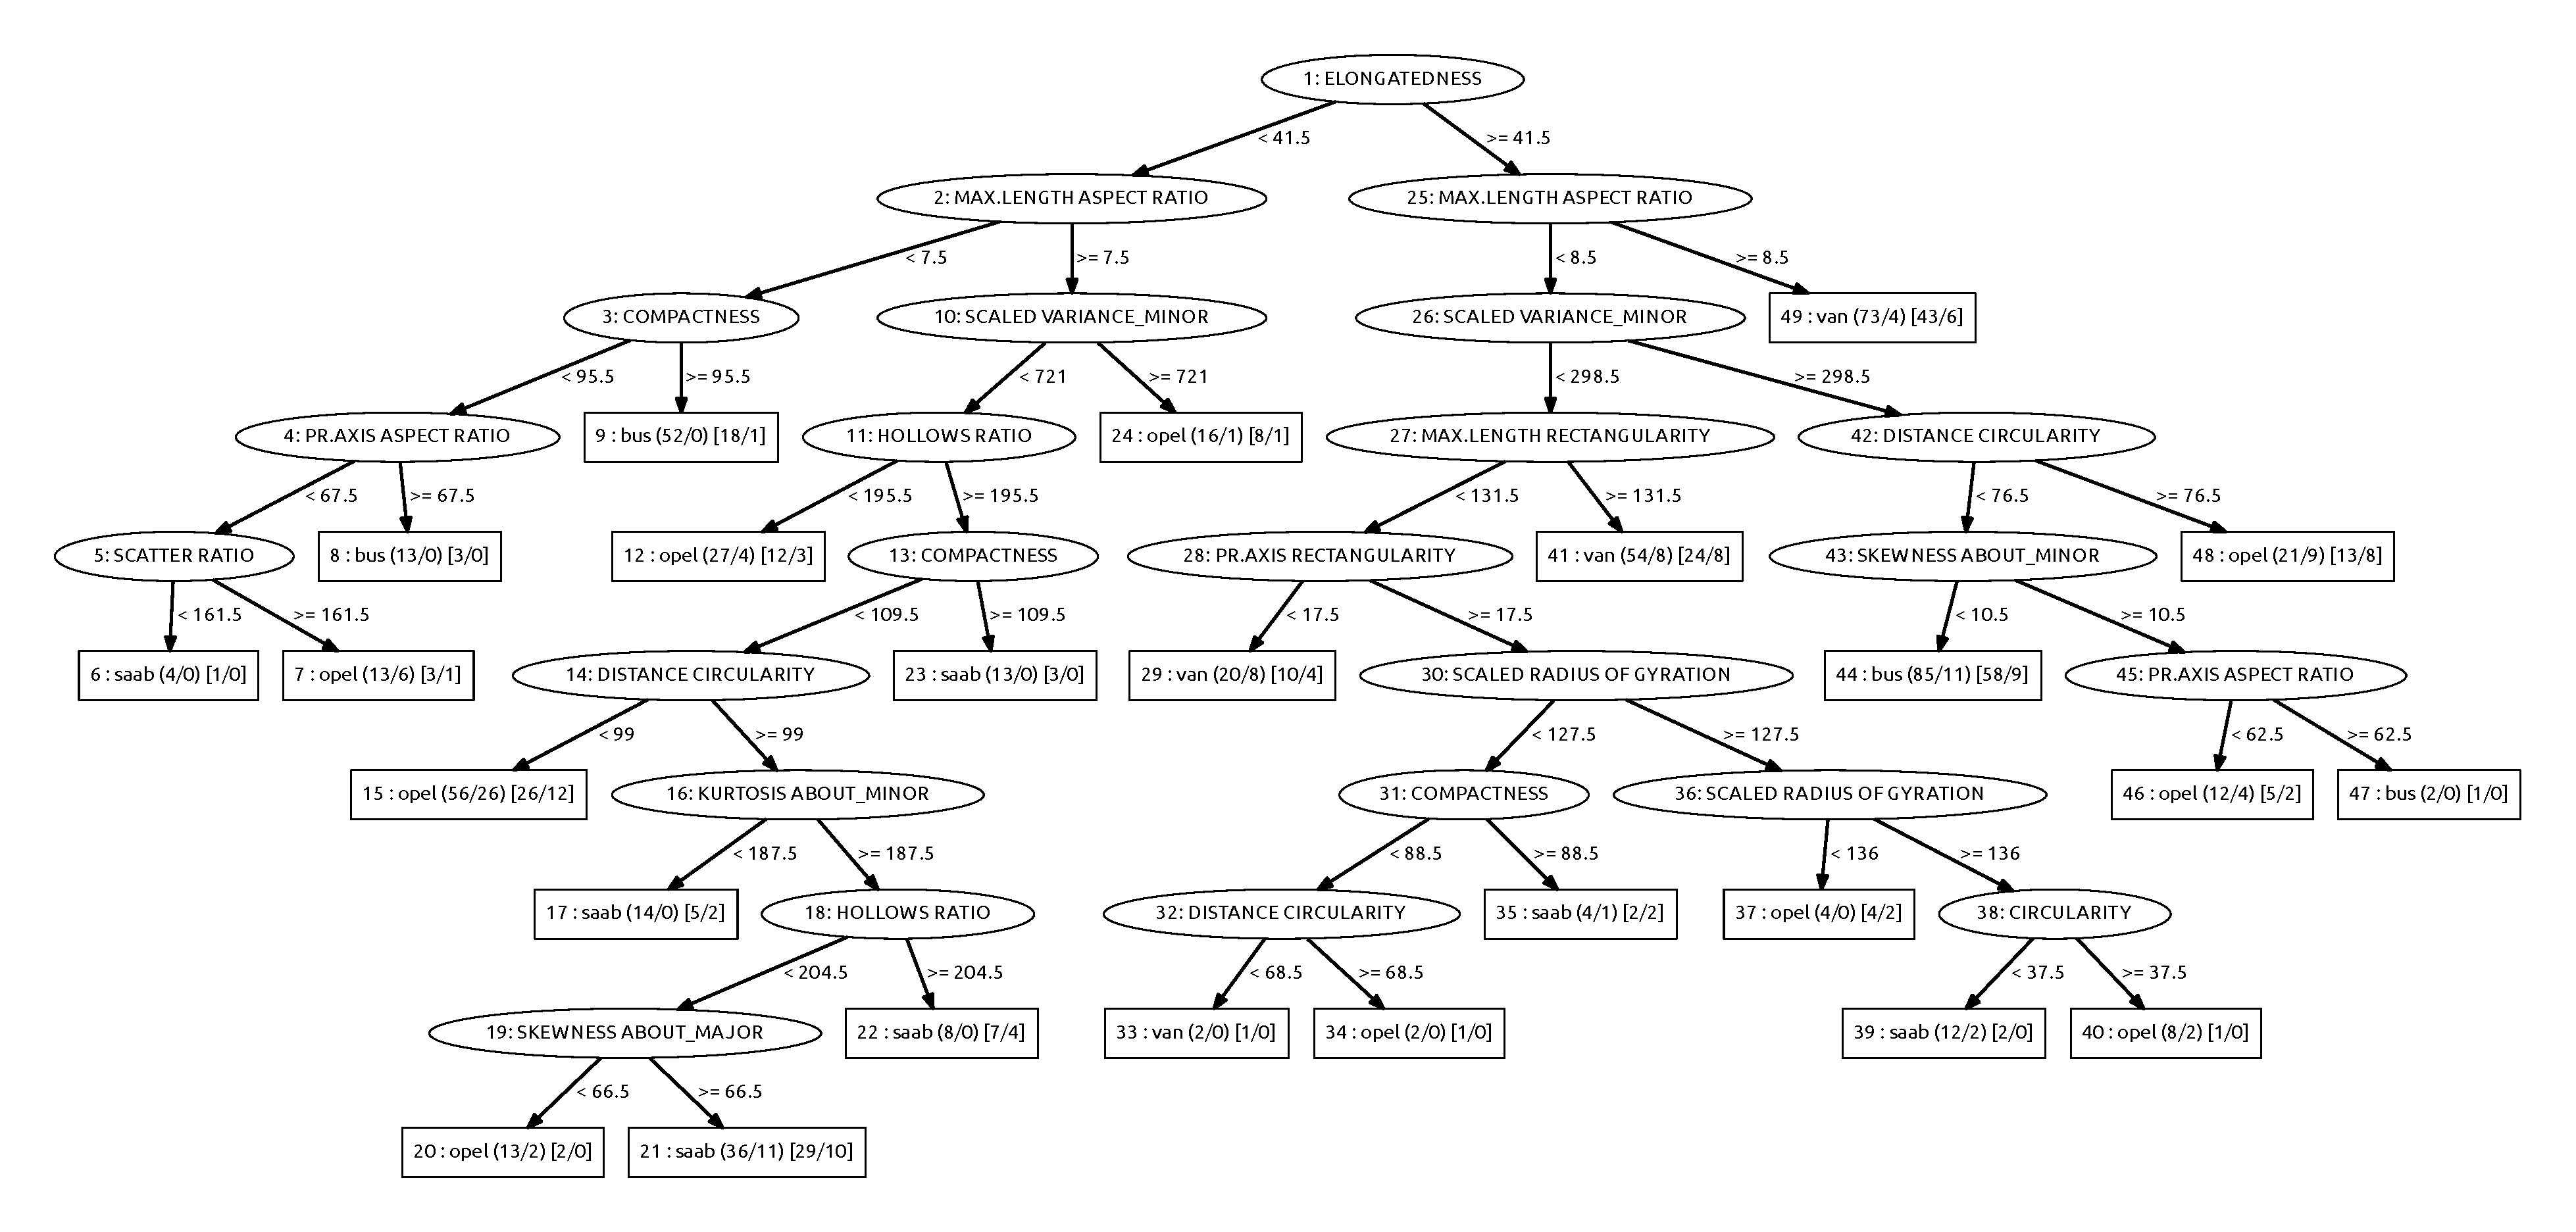
\includegraphics[width=1.55\textwidth]{results/reptree/vehicle.pdf}}
	\caption{Modello di REPTree}
\end{figure}

\begin{mdframed}[frametitle=Esecuzione JRip]
	\scriptsize\verbatiminput{results/jrip/vehicle.jrip}
\end{mdframed}

%\begin{adjustwidth}{-8em}{}
%	\scriptsize\verbatimtabinput{results/jrip/vehicle.rules}
%\end{adjustwidth}

\vspace{-2em}
\begin{mdframed}[frametitle=Regole]
	\begin{adjustwidth}{.3\linewidth}{}
		\scriptsize\verbatimtabinput{results/jrip/vehicle.rules}
	\end{adjustwidth}
\end{mdframed}

\pagebreak

\section{Risultati su \texttt{Wisconsin Breast Cancer}}

\begin{mdframed}[frametitle=Esecuzione REPTree]
	\footnotesize\verbatiminput{results/reptree/wisconsin_breast_cancer.reptree}
\end{mdframed}

\begin{figure}[htb]
	\vspace{-2em}
	\makebox[\textwidth]{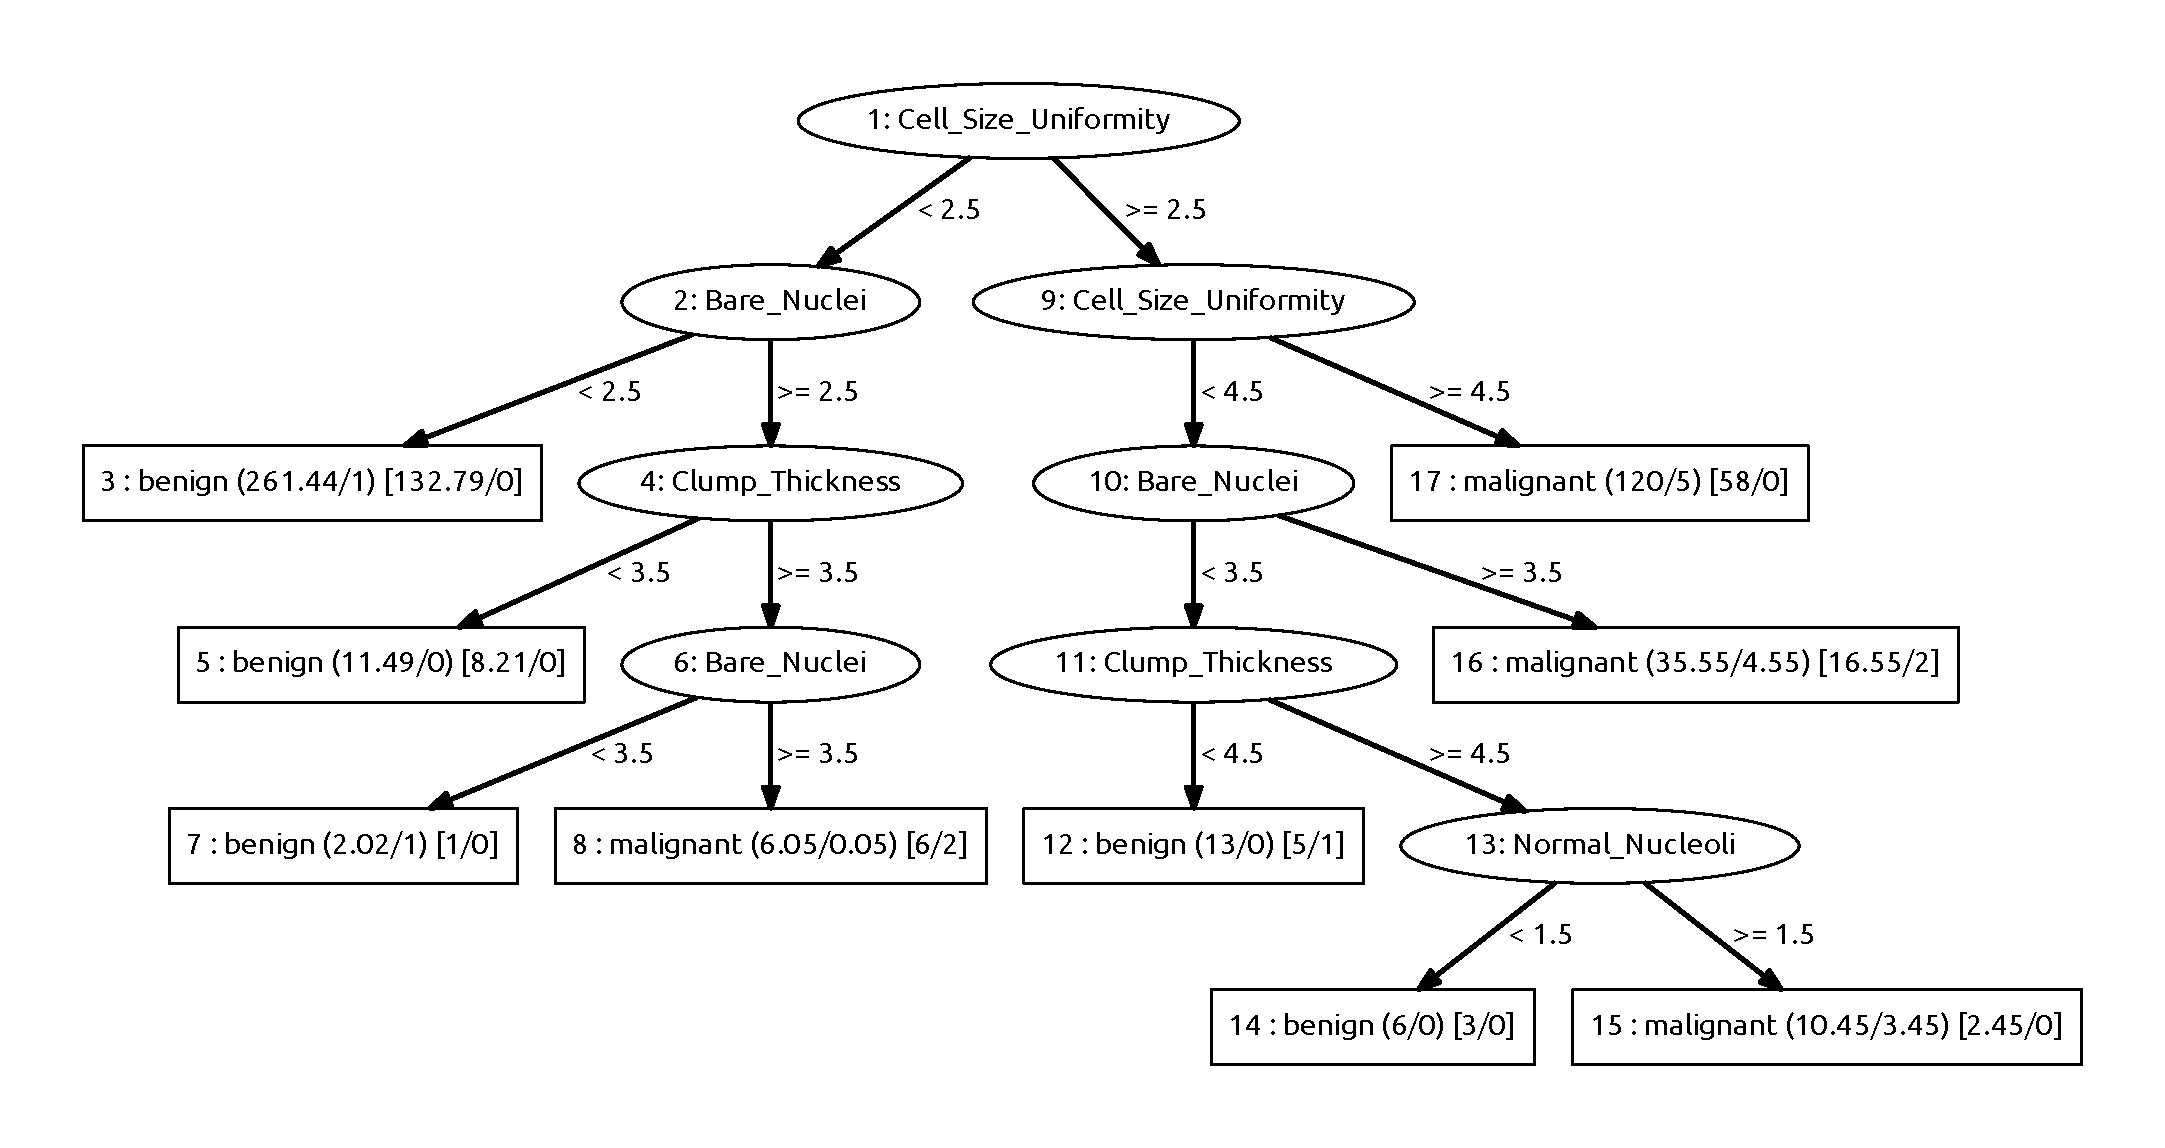
\includegraphics[width=1.55\textwidth]{results/reptree/wisconsin_breast_cancer.pdf}}
	\caption{Modello di REPTree}
\end{figure}

\begin{mdframed}[frametitle=Esecuzione JRip]
	\footnotesize\verbatiminput{results/jrip/wisconsin_breast_cancer.jrip}
\end{mdframed}

\vspace{-2em}
\begin{mdframed}[frametitle=Regole]
	\begin{adjustwidth}{.3\linewidth}{}
		\footnotesize\verbatimtabinput{results/jrip/wisconsin_breast_cancer.rules}
	\end{adjustwidth}
\end{mdframed}

%\footnotesize\verbatimtabinput{results/jrip/wisconsin_breast_cancer.rules}